\section*{Sense and avoid for small UAV}
Unmanned Aircraft Vehicles (UAV) are increasingly used for a number of civil and military applications. 
In particular, small size UAV are capable of delivering sensing and communication services for a fraction of the cost of bigger UAVs or of manned aircraft. This is because of simpler operational logistics and maintenance. 
To carry out a variety of tasks it is necessary to safely integrate UAV's into non-segregated airspace.
Cooperative and non cooperative Sense and Avoid (SAA) systems are key enablers for Unmanned Aircraft (UAV) to
routinely access non-segregated airspace \cite{spriesterbach2013unmanned}.
Both cooperative and non-cooperative SAA systems are being developed to address this integration requirement.

The SAA capability is defined as the automatic detection of possible conflicts by the UAV platform under
consideration and performing avoidance maneuver tasks to prevent the identified collisions.
An analysis of the available SAA candidate technologies and the associated
sensors for both cooperative and non-cooperative SAA systems is presented in \cite{muraru2011critical}.
Non-cooperative Collision Detection and Resolution (CD\&R) for UAV is considered as one of the major challenges that needs to be addressed \cite{lai2012see} for the insertion of UAVs in non-segregated air space.
As a result, a number of non-cooperative sensors for the SAA system have been adopted. Light Detection and Ranging (LIDAR)is used for
detecting, warning and avoiding obstacles for low-level flying \cite{sabatini2014lidar}.

An approach to the definition of encounter models and their applications to SAA strategies is presented in \cite{kochenderfer2008encounter} for both cooperative and non-cooperative scenarios.

Since 2014, there is a visible strong political support for developing rules on drones but regulations are not harmonized yet. The European Aviation Safety Agency (EASA) has been tasked to develop a regulatory framework for drone operations and proposals for the regulation of "low-risk" UAV operations. In achieving this, EASA is working closely with the Joint Authorities for Regulation of Unmanned Systes (JARUS) \cite{jarus2016regulations}.

The development of SAA systems for small UAV presents added challenges because of the size, power, and weight limitations. These limitations preclude the use of SAA systems developed for manned aircraft or for bigger UAV. New sensing and avoidance technologies are needed to address these challenges. This is the goal of this work.


\section*{Approach}\label{ch:approach}
The proposed approach combines \textit{LiDAR} sensing technology with techniques based on controlled invariance. \textit{LiDAR} provides a point-cloud representation of the world in the field of view of the sensor. Controlled invariance techniques provide a characterization of flight envelopes that by design avoid obstacles under reasonable assumptions. 

The approach presents a nested solution to control design depicted in Figure \ref{fig:ControlConcept}. There is a nominal trajectory for the UAV that may be generated by an  \textit{Optimal trajectory control} module, for example. The \textit{LiDAR} sensor will continuously scan the environment for obstacles. If an obstacle crosses a pre-computed safety zone then an \textit{Emergency avoidance module} is invoked to override the trajectory tracking controller. The safety zone is computed using invariance techniques based on reach set computations. When the obstacle no longer presents a threat (i.e., it does not belong to the safety zone) control is returned to \textit{Optimal trajectory control} module. This nested control approach entails  a \textit{Control strategy switch} will override control input of system and starts avoidance maneuver to achieve \textit{reactive avoidance}.
 
\begin{figure}[H]
    \centering
    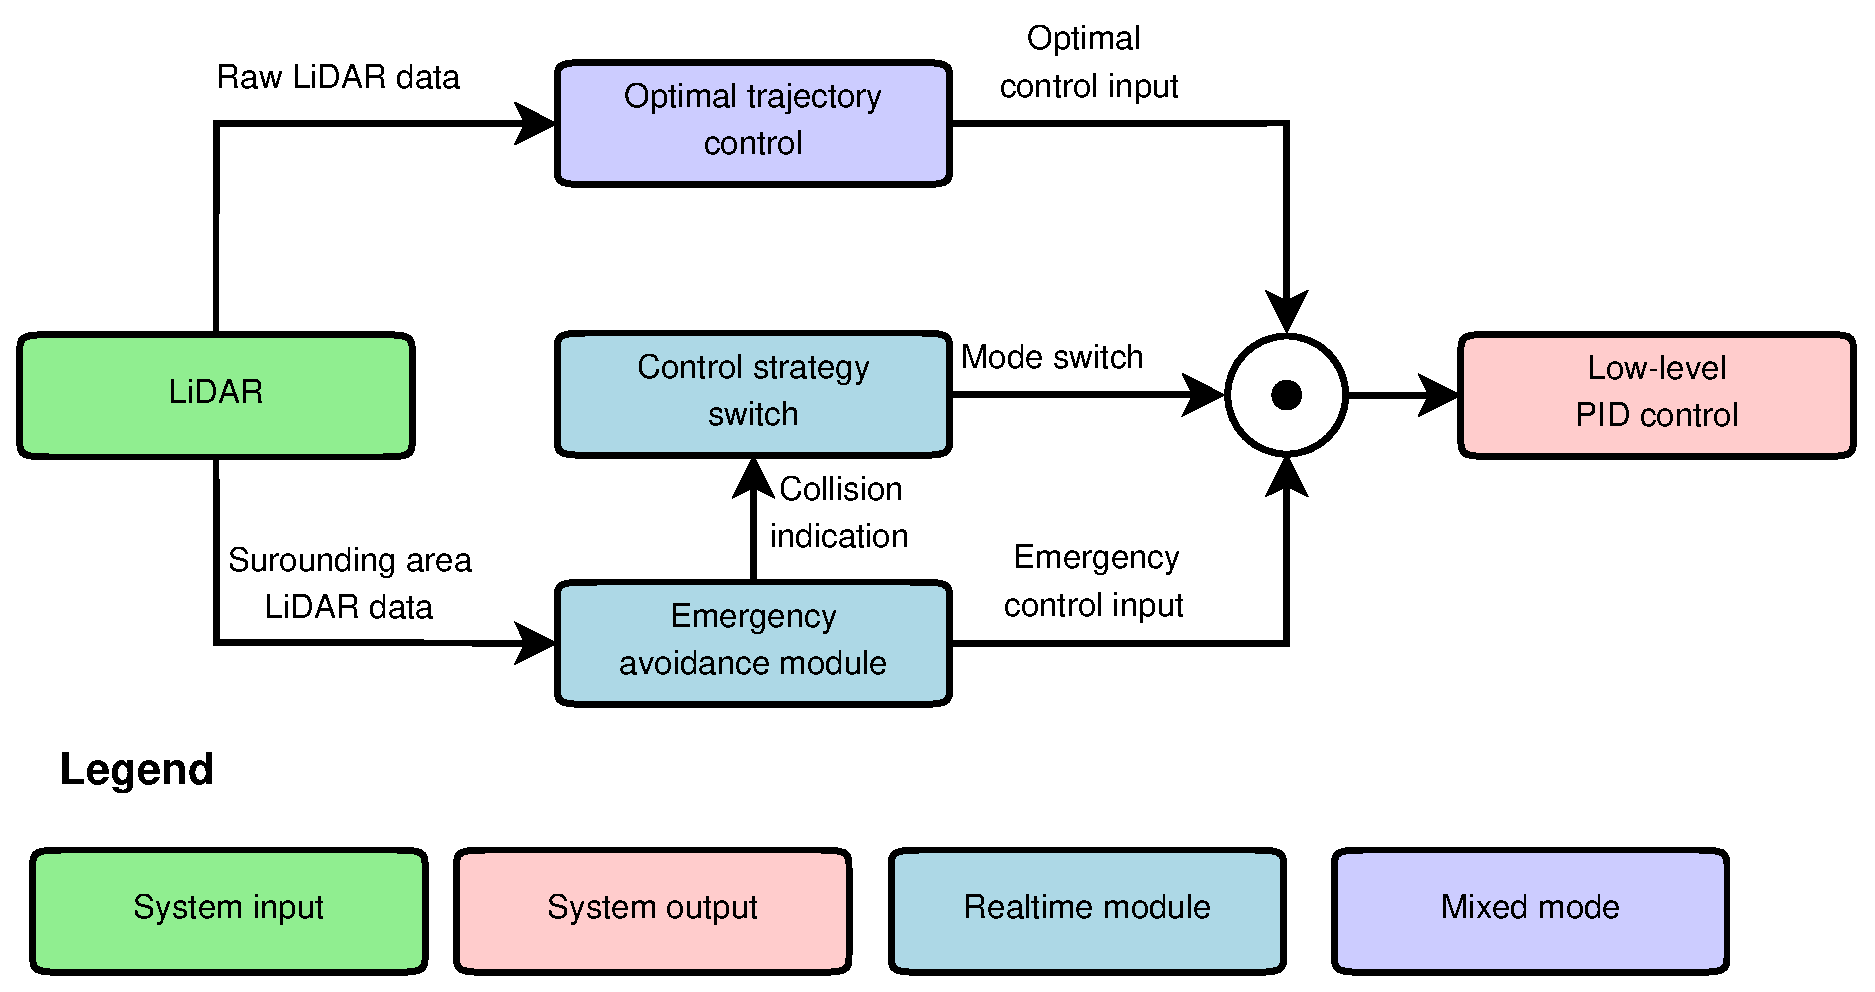
\includegraphics[width=10cm]{Pics/35_ControlConcept.eps}
    \caption{Control concept scheme}
    \label{fig:ControlConcept}
\end{figure}


\section*{Goals}

The goal of the research is to develop an integrated approach to real-time obstacle detection and avoidance for Unmanned Air Vehicles (UAV) based on \textit{LiDAR} technology. The approach concerns the solution of the following sub-problems:
\begin{enumerate}


    \item  \textit{Obstacle detection and sensor fusion} - processing \textit{LiDAR} data into an unified and compact data representation for obstacle detection. 
		
    \item  \textit{Real-time reactive obstacle avoidance} - identify safety problems and perform avoidance maneuvers with safety guarantees when collisions are possible and return control to nominal controller when collision is avoided.

\end{enumerate}


The following assumptions are considered in this work:
\begin{enumerate}
	\item There is a real-time point cloud representation of LiDAR data (with some degree of uncertainty).
	\item There is an a-priory global terrain map, which may change with time.
	\item There are no moving obstacles.
	\item Estimates of the state of the UAV are available.
	\item The operational space does not contain 'traps' such as caves. 'Traps' arise because the field of view of the LIDAR does not include the whole space surrounding the UAV.
	\item There is a mission plan for the UAV consisting of a trajectory, which may be optimal or not.
\end{enumerate}

A formal approach to this problem will be developed with focus on performance and safety guarantees for real-time operations. The approach will be flight tested on an UAV which will also be designed and built in the context of this work.


\section*{Research plan}

The research plan will be organized around the following tasks:

\textit{Reachable space estimation in partially known space} - research of reachable space with strong/weak invariance estimation during flight. Method will place importance on fast calculation of reachable space enriching space occupied by obstacles. This enrichment will enable to calculate accurate avoidance trajectories with optimal cost. The technical approach will be based on reach set computations and invariance techniques INCLUDE REFERENCES AND ELABORATE A BIT MORE ON THIS

\textit{Avoidance theorem formulation} - multiple parameters needs to be taken into consideration before avoidance maneuver execution. Most of previous work have been considering only technical aspects of obstacle avoidance. Main goal of thesis will be to build abstract avoidance framework. Theorem will take into account various aspect ranging from technical aspects to statistical errors during flight. The technical approach will be based on reach set computations and invariance techniques INCLUDE REFERENCES AND ELABORATE A BIT MORE ON THIS


\textit{Compact object approximation in partially known space} - research of feasible representation of obstacles in partially known space. \textit{LiDAR} output is usually very thick in terms of data flow. It is not feasible to work with all measured data. Computer vision offers various methods to represent thick point cloud as compact surfaces. Potential contribution is to enrich these methods to work near real-time with streamline input. The technical approach will be based on XXX INCLUDE REFERENCES AND ELABORATE A BIT MORE ON THIS

\textit{Simulations} - develop a computational simulation environment to test and evaluate the overall approach. This will be implemented with the help of the LSTS software toolchain and will support hardware-in-the-loop simulations. A thorough test plan will be targeted at exercising the overall approach in a representative sample of flight conditions.

\textit{Flight tests} - develop a UAV based on an n-copter to flight test the approach. The test plan will exercise a representative sample of the simulation test plan. 

These tasks will be developed incrementally to minimize risk. This means that each task will be decomposed into several subtasks of increasing complexity. Each subtask will produce meaningful and useful results and will provide insights regarding the solution of more complex subtasks. 



